\subparagraph*{Submission : }
\textit{Do the same as Step 6 when the conversion rates are not stationary. Adopt a change-detection test approach.}\\

The goal is the same of the previous problem, but instead of a sliding-window approach, is required to adopt a change-detection test approach.

\subsection*{Basic knowledge}
\subparagraph*{Change Detection (CUSUM)}
The first $M$ valid samples are used to produce the reference point.\\

Empirical mean of arm $a$ over the first $M$ valid samples $\bar{X_{a}^0}$\\

From the $M + 1-th$ valid sample on, we check whether there is a change\\

Positive deviation from the reference point at $t$ \hspace{0.2cm} $s_{a}^{+}(t) = (x_{a}(t) - \bar{X_{a}^0}(t)) - \epsilon$ \\

Negative deviation from the reference point at $t$ \hspace{0.2cm} $s_{a}^{-}(t) = -  (x_{a}(t) - \bar{X_{a}^0}(t)) - \epsilon$ \\

Cumulative positive deviation from the reference point at $t$ \hspace{0.2cm} $g_{a}^{+}(t) = \max \left\{0, g_{a}^{+}(t-1) + s_{a}^{+}(t) \right\}$ \\

Cumulative negative deviation from the reference point at $t$ \hspace{0.2cm} $g_{a}^{-}(t) = \max \left\{0, g_{a}^{-}(t-1) + s_{a}^{-}(t) \right\}$ \\

We have a change if \hspace{0.2cm} $g_{a}^{-}(t) > h$ or $g_{a}^{+}(t) > h$\\
\subparagraph*{CD-UCB}

\textbf{Pseudocode:}\\

1. Initialize $\tau_{a} = 0$ for $a\in A$ 

2. For each time $t$:\\

\hspace{0.8cm} $a_{t} \leftarrow \argmax_{a \in A}{\left\{\bar{x}_{a,\tau_{a},t} + \sqrt{\frac{2 log(n(t))}{{n_{a}(\tau_{a},t-1)}} }\right\}}$ with probability $1-\alpha$\\

\hspace{0.8cm} $a_{t} \leftarrow$ random arm with probability $1-\alpha$ \\

$n(t)$	is total number of valid samples\\

$\bar{x}_{a,\tau_{a},t}$ is the empirical mean of arm $a$ over the last valid samples\\

$n_{a}(\tau_{a},t-1)$ is the number of valid samples for arm $a$\\

3. Collect reward $r_t$\\

4. If $CD_a (r_{\tau},...,r_t) = 1$ then $\tau_a = t$ and restart $CD_a$


\subsection*{Strategy}
In order to solve this problem we have used a change detection (CUSUM) algorithm and a bandit algorithm (UCB). At each time $t$, the UCB outputs a decision $I_t \in K$, where $K$ is a set of arms, based on its past observations of the bandit environment. The environment generates the corresponding reward of arm $I_t$, which is observed by both the bandit algorithm and the change detection algorithm. The change detection algorithm monitors the distribution of each arm, and sends out a positive signal to restart the bandit algorithm once a breakpoint is detected.

\subparagraph{Implementation}
\begin{itemize}
	\item Three seasons: Spring-Summer, Autumn, Winter
	\item Number of customers per class is not known 
	\item Candidates for the \textit{Racing Skis} are: \{2110.0, 1900.0, 2420.0, 2690.00\}
	\item Candidates for the \textit{Racing Ski Helmet} are: \{360.0, 410.0, 530.0, 600.0\}
	\item Conversion rate associated with the first item is not known
	\item Conversion rate associated with the second item is not known
	\item Promotion assignment is not known 
	\item Change-detection test approach
\end{itemize} 

\subparagraph{Optimal strategy}
We have calculate the optimal solution in the same way as in the point 6. The only difference is that we will have one optimal solution per season, so at the beginning of each of them we have to calculate it again.
According to our candidates the optimal solution is:

\begin{center}
	\begin{tabular}{|c|p{4cm}|p{4cm}|p{4cm}|} 
		\hline
		Season & \textit{Racing Skis optimal price} & \textit{Racing Ski Helmet} optimal price & Optimal promo-category matching \\ \hline
		\multirow{4}{*}{Spring-Summer} & \multirow{4}{*}{1900.0} & \multirow{4}{*}{360.0} & Sport addicted: P$_0$ = 0\% (360.0)  \\ 
		& 					   &                      & Gifted: P$_1$ = 10\% (324.0)          \\ 
		& 					   &                      & Worried: P$_2$ = 20\% (288.0)         \\
		& 					   &                      & Amateur: P$_3$ = 30\% (251.99)         \\ \hline
		\multirow{4}{*}{Autumn} & \multirow{4}{*}{2690.0} & \multirow{4}{*}{530.0}  & Sport addicted: P$_1$ = 10\% (477.0)\\ 
		& 					   &                      & Gifted: P$_3$ = 30\% (371.0)         \\ 
		& 					   &                      & Worried: P$_2$ = 20\% (424.0)         \\
		& 					   &                      & Amateur: P$_0$ = 0\% (530.0)         \\ \hline
		\multirow{4}{*}{Winter} & \multirow{4}{*}{2420.0} & \multirow{4}{*}{600.0}  & Sport addicted: P$_3$ = 30\% (420.0)\\ 
		& 					   &                      & Gifted: P$_1$ = 10\% (540.0)         \\ 
		& 					   &                      & Worried: P$_2$ = 20\% (480.0)         \\
		& 					   &                      & Amateur: P$_0$ = 0\% (600.0)          \\ \hline
	\end{tabular}
\end{center}

Days: 365\\
Experiments number: 2 \\





\subsection*{Results}
\begin{center}
	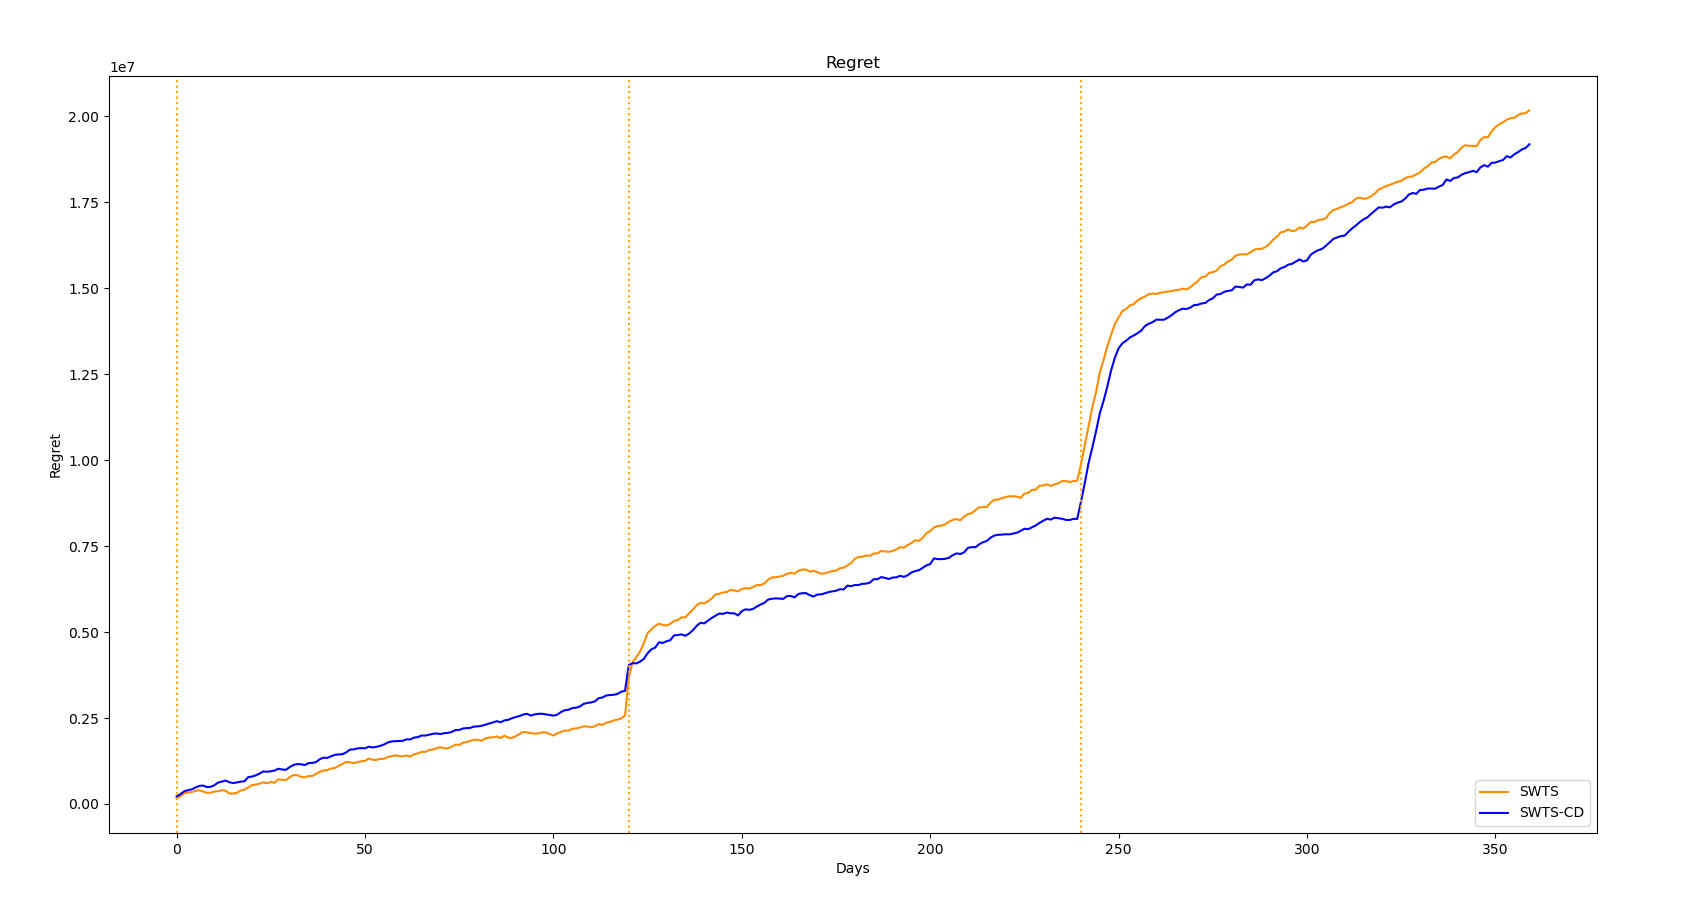
\includegraphics[scale=0.35]{Images/n8}
\end{center}
\subsection*{Considerations}
We can observe that the change-detection approach has a small impact respect to the performance of the SW-TS. This is due to the fact that the change-detection approach catches some false-positive detection; the matching of promo-category of the second item is influenced by the prices chosen for the two items.
